\documentclass[]{article}
\usepackage{graphicx}
%opening
\title{ Report for Artificial Intelligence }
\author{ Simone D'Antimo, Francesco Caldivezzi, Harjot Singh}
\graphicspath{ {./images/} }

\begin{document}

\maketitle

\begin{abstract}
Coronavirus disease (COVID-19) has significantly affected the daily life activities of people globally.
To prevent the spread of COVID-19, the World Health Organization has recommended people to wear face masks in public places.
Manual inspection of people for wearing face masks in public places is a challenging task.

The program we have implemented had 2 important parts: 
The first one is to recognize the face of a person, and to do that we use python with opencv libraries.

The second part of our project regards the model we use to estimate if a person is wearing a mask. We used the RES-Net 50 convolution neural network to create and train our model. Since the model created is very heavy we had to fine-tune it in order to implement it in our program.

The RES-Net 50 model that we created works really well with the dataset that we have used. We split data in 60 - 20 - 20 train-validation-test and the accuracy of the test set is 0.98.

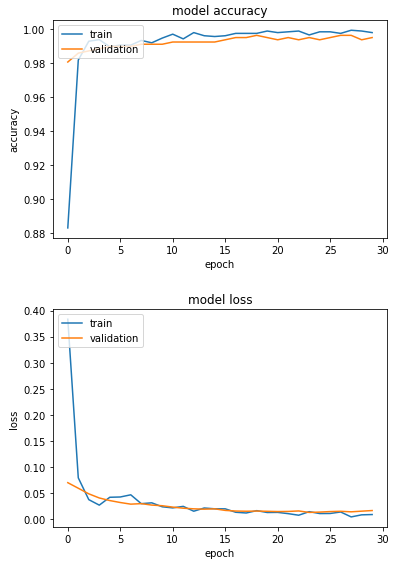
\includegraphics{LossAndAccuracy}

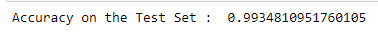
\includegraphics{testAccuracy}

roba usata per il crop dell'immagine, (?) 

conclusioni


Future works:
Since our model is heavy, also the fine-tuned one, it is possible that not all the device are able to compute it in a reasonable amount of time, In order to develop a program that may be used in a more heterogeneous amount of device we have found other models, thinner than Resnet50, that may be implemented to scan face faster. This model is called MobileN.
riferimenti bibliografici ai paper letti

\end{abstract}

\section{}

\end{document}
